\subsubsection{Elección de microcontrolador} \mbox{} \vspace{10pt} \\
Dentro de las características del modelo anterior de la familia Hermes, se destacaba la gran cantidad hardware por el cual estaba compuesto, y por ende, el gran costo para su replicación e implementación.

Para esta nueva edición se decidió reducir la cantidad de componentes que lo integran, en cuanto al procesamiento se refiere, y llevarlo a un modelo que se acerque mas a la Industria 4.0 donde los dispositivos se conectan a Internet y es allí donde mandan reportes y reciben instrucciones. Es por eso que se optó por la utilización del microcontrolador ESP-32 el cual proporciona un API bastante completa y por en ende un gran abanico para que el desarrollador despliegue todo su potencial.

\begin{figure}[H]
   \centering
   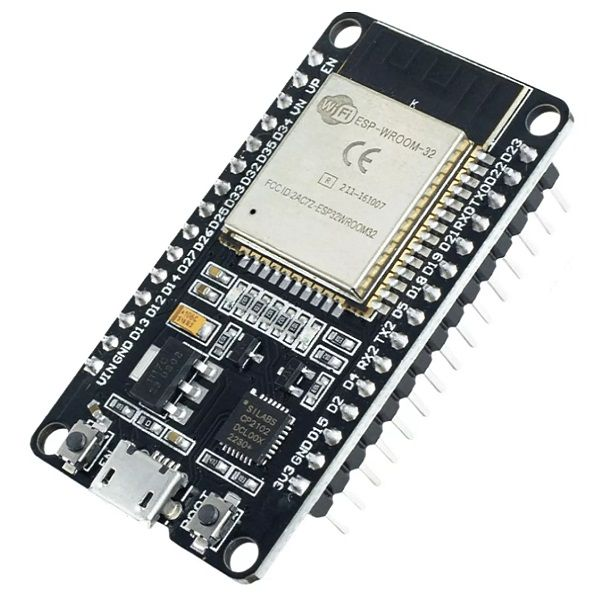
\includegraphics[width=0.4\linewidth]{images/esp32.jpeg}
   \caption{Microcontrolador ESP32}
   \label{fig:microcontrolador}
\end{figure}